% CVSId: $Id: oqe.tex,v 1.12 2002-05-07 01:20:03 cananian Exp $
\documentclass[%
pdf,
colorBG,
slideColor,
%nocolorBG,
%slideBW,
%%%%%%%%%%%%%%%%%%%%%
nototal,
%distiller,
%%%%%%%%%%%%%%%%%%%%%
%draft,
oqe
%frames
%azure
%contemporain
%nuancegris
%troispoints
%lignesbleues
%darkblue
%alienglow
%autumn
]{prosper}
\usepackage{amsmath}
\usepackage{comdef}\newcommand{\figscale}{1.0}
\usepackage{pst-node}
\usepackage{verbatim}
%\hypersetup{pdfpagemode=FullScreen}

\title{Size Optimizations for Java Programs}
%\author{\href{http://cscott.net}{C.~Scott~Ananian}}
\author{C.~Scott~Ananian}
\email{cananian@lcs.mit.edu}
\institution{%
Laboratory for Computer Science\\
Massachusetts Institute of Technology}

%\DefaultTransition{Wipe}
\renewcommand{\yellow}{\colC}
\ifDVItoPS\renewcommand{\white}{\black}\fi
\newcommand{\betweenSlide}[3]{\fromSlide{#1}{\untilSlide{#2}{#3}}}
\newenvironment{mysamplecode}{\small\bfseries\begin{samplecode}}{\end{samplecode}}
% Meet symbol
\newcommand{\meet}{\ensuremath{\sqcap}}
% lattice inequalities
\newcommand{\latlt}{\ensuremath{\sqsubset}}
\newcommand{\latleq}{\ensuremath{\sqsubseteq}}

%%%%% define new 'talknotes' environment that only shows up in PS mode.
\ifDVItoPS
\newenvironment{talknotes}{\begin{slide}{Notes}\tiny}{\end{slide}}
\else
% this redefinition of talknote to be == comment is from an example in
% the verbatim package (where the comment environment comes from).
\let\talknotes=\comment
\let\endtalknotes=\endcomment
\fi

\begin{document}
\maketitle

\begin{talknotes}
Nothing should be said on the title slide.
\end{talknotes}

%---------------------------------------------------------------------- SLIDE -
% \begin{slide}{The quest for $\pi$}
% \begin{itemize}
% \item The following formula computes $8$ correct digits per iteration 
%   (Ramanujan):
% \end{itemize}
%   \begin{small}
%   \begin{equation*}
%     \frac{1}{\pi}=\sum_{n=0}^\infty \frac{(\frac{1}{4})_n(\frac{2}{4})_n(\frac{3}{4})_n}{n!^3}\bigl(2\sqrt{2}(1103+26390n)\bigr)\frac{1}{(99^2)^{2n+1}}
%   \end{equation*}
%   \end{small}
% \end{slide}

%---------------------------------------------------------------------- SLIDE -
\begin{slide}{Our Goal}
\begin{center}
Reduce the memory consumption of object-oriented programs

\vspace{0.5cm}
\fontTitle{By}
\vspace{0.5cm}

Using program analysis to identify opportunities to reduce the space
required to store objects,

\vspace{0.5cm}
\fontTitle{Then}
\vspace{0.5cm}

Applying transformations to reduce the memory consumption of the program.
\end{center}
\end{slide}

\begin{talknotes}
This talk is about size optimizations for Java programs.  Our goal is
to reduce the amount of memory used by object-oriented programs (in
this case, Java) by using static whole-program analyses to identify
opportunities and applying transformations to effect the reduction.
\end{talknotes}

%---------------------------------------------------------------------- SLIDE -
\begin{slide}{Structure of a Java Object}
\begin{itemize}
\item Typical of many O-O languages.
\end{itemize}
\begin{center}
\includegraphics[scale=0.5]{Figures/Kontour/structure-bbox.eps}
\end{center}
\end{slide}

\begin{talknotes}
Here's our starting point.  This is how most Java implementations lay
out objects.  I want you to notice that there are three kinds of space
in this layout, helpfully delineated with red lines.  The first
section of the object usually consists of information required by
the runtime implementation but not directly specified by the
programmer.  This includes a claz pointer, which points to an
external structure of information about the object's type, and
some information to support the hashcode and locking semantics of
Java.  Every object has a hashcode and can be locked upon, etc, etc.
The second section of the object contains the fields declared by
the programmer.  If this were a car object, these fields might
indicate the color and model of the car.  The last section
consists of padding which the runtime implementation will
add to bring the various parts of the object to certain alignment
boundaries.
\end{talknotes}

%---------------------------------------------------------------------- SLIDE -
\overlays{2}{
\begin{slide}{Strategy}
\fromSlide{2}{
\begin{center}
Push hard on all the bits.

\vspace{0.5cm}
\includegraphics[scale=0.5]{Figures/Kontour/strategy-bbox.eps}
\end{center}
}
\end{slide}
}

\begin{talknotes}
Our strategy is simple: @ we're going to push hard on all the bits,
in the object header, in the fields of the object, and even on the
padding bytes, in order to reduce the size of each object and thus
the total allocated and live memory of the program.
\end{talknotes}

%---------------------------------------------------------------------- SLIDE -
\newrgbcolor{fieldcomp}{0 1 0}
\newrgbcolor{fieldelim}{0 1 1}
\newrgbcolor{headeropt}{1 0 0}

\overlays{4}{
\begin{slide}{How to compress objects}

Three broad techniques:
%
\parbox[b]{2.5in}{%
\fromSlide{2}{
\begin{itemize}%
\fieldcomp\renewcommand{\green}{\fieldcomp}% new bullet color
\item Field compression
\fromSlide{3}{
\fieldelim\renewcommand{\green}{\fieldelim}% new bullet color
\item Mostly-constant field elimination
\fromSlide{4}{
\headeropt\renewcommand{\green}{\headeropt}% new bullet color
\item Header optimizations
}}
\renewcommand{\green}{\yellow} % restore yellow bullet color
\end{itemize}
}}%
\parbox[b]{1.75in}{%
\onlySlide*{1}{\hspace*{0.106in}\hspace*{0.261in}\includegraphics[scale=0.4]{Figures/Kontour/how-none-bbox.eps}}%
\onlySlide*{2}{\hspace*{0.106in}\hspace*{0.261in}\includegraphics[scale=0.4]{Figures/Kontour/how-fieldcomp-bbox.eps}}%
\onlySlide*{3}{\hspace*{0.106in}\includegraphics[scale=0.4]{Figures/Kontour/how-fieldelim-bbox.eps}}%
\onlySlide*{4}{\includegraphics[scale=0.4]{Figures/Kontour/how-header-bbox.eps}}%
}%

\end{slide}
}

\begin{talknotes}
There are three broad techniques we are going to use to effect our
size reductions: @ field compression, @ mostly-constant field
elimination, and @ header optimizations.  We will look at each
of these in order, starting with\ldots
\end{talknotes}

%---------------------------------------------------------------------- SLIDE -
\begin{slide}{How to compress objects} % just the first one

Three broad techniques:

\parbox[b]{2.5in}{%
\begin{itemize}%
\fieldcomp\renewcommand{\green}{\fieldcomp}% new bullet color
\item Field compression
\lightgray\renewcommand{\green}{\lightgray}% new bullet color
\item Mostly-constant field elimination
\lightgray\renewcommand{\green}{\lightgray}% new bullet color
\item Header optimizations
\renewcommand{\green}{\yellow} % restore yellow bullet color
\end{itemize}
}%
\parbox[b]{1.75in}{%
\hspace*{0.106in}\hspace*{0.261in}\includegraphics[scale=0.4]{Figures/Kontour/how-fieldcomp-bbox.eps}%
}%
\end{slide}

\begin{talknotes}
\ldots field compression.
\end{talknotes}

%---------------------------------------------------------------------- SLIDE -
\overlays{6}{
\begin{slide}{Field Compression}
Reduce the space taken up by an object's fields.
\begin{itemize}
\fromSlide{2}{
\item \bp{\yellow Sparse Predicated Typed Constant analysis} to
  discover unread/unused/constant fields.
\fromSlide{4}{
\item \bp{\yellow Bitwidth analysis} to discover tight upper bounds on
  field size.
\fromSlide{6}{
\item \bp{\yellow Field packing} into bytes or bits.
}}}
\end{itemize}

\framebox{\parbox{2in}{%
\begin{mysamplecode}%
class Car \{\\
\>int color;\\
\>\ldots\\
\}\\
\end{mysamplecode}%
}%
\parbox{3in}{%
\fromSlide{3}{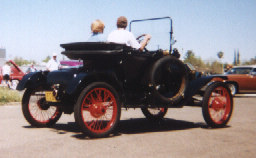
\includegraphics[height=.8in]{Figures/Images/model-t-black.eps}}
\fromSlide{5}{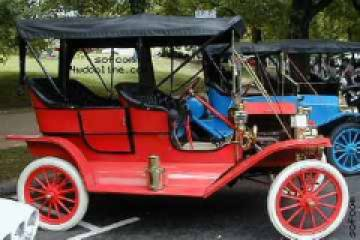
\includegraphics[height=.8in]{Figures/Images/model-t-redblue.eps}}\\
\tt\bfseries%
~\fromSlide{3}{{\black BLACK=0}}%
~\fromSlide{5}{{\red RED=1}~{\blue BLUE=2}}
}%
}

\end{slide}
}

\begin{talknotes}
Field compression targets the space directly allocated by the
programmer.  In the sample class at the bottom of the slide, we
define an object representing cars.  It's first field is a color,
and it is declared an integer which allows the enumeration of up
to $2^{32}$ different colors of cars.
%
@ The first analysis we do is a standard sparse conditional constant
propagation pass over the whole program to identify unused, unread,
or constant fields.  @ Suppose we're building Ford Model-T's.
Since they only come in black, this field will be constant and
can be removed.
%
@ The novel contribution is the next step, bitwidth analysis, which discovers
tigher upper bounds on field sizes.  @  Actually, Model-T's were
produced in several different colors before Ford started
mass-production.  Our bitwidth analysis could determine that
we really only need two bits to store colors, since our program
only ever stores three different colors in a Car.
%
@ After we perform the analysis, we use the results to
reduce the padding between fields.  We'll talk about this later.
\end{talknotes}

%---------------------------------------------------------------------- SLIDE -
\overlays{10}{
\begin{slide}{Intraprocedural SPTC Example}
\begin{center}%
\parbox[c]{2in}{%
\begin{mysamplecode}%
int foo() \{\\
\>if (\ldots)\\
\>\>\betweenSlide{4}{6}{\yellow}i=1;\\
\>else\\
\>\>\betweenSlide{7}{9}{\yellow}i=2;\\
\>\onlySlide{10}{\yellow}if (i>0)\\
\>\>$\vdots$\\
\}\\
\end{mysamplecode}%
}%
\parbox[c]{2.6in}{%
\fromSlide{2}{%
\begin{center}
\renewcommand{\figscale}{0.6}%
\newcommand{\color}[2][rgb]{}%ignore color commands
\input{Figures/THlat1b}
\end{center}
}}

\fromSlide{3}{\framebox{$\text{\tt\bfseries i} =
    \untilSlide*{4}{\bot}%
    \onlySlide*{5}{\bot\yellow\meet 1}%
    \onlySlide*{6}{\yellow 1}%
    \onlySlide*{7}{1}%
    \onlySlide*{8}{1\yellow\meet 2}%
    \fromSlide*{9}{1\meet 2\onlySlide{9}{\yellow}=\top}%
    $}}

\vspace{.5cm}
\onlySlide*{6}{[Because $\bot \latleq 1$ and $1 \latleq 1$]}
\fromSlide*{9}{[Because $1 \latleq \top$ and $2 \latleq \top$]}
\end{center}
\end{slide}
}

\begin{talknotes}
Let's look at a quick example of how the Sparse Predicated Typed
Constant analysis is done. @ We have this simple program, which
assigns values to an integer variable {\tt i} and then tests the
result.  @ When we perform the dataflow analysis, we will abstract the
value domain of the program using this lattice of integer
constants.  The $\bot$ value indicates that nothing is known about the
value of a variable. @ At the start of the analysis, we know nothing
about the value of {\tt i}. @ When the analysis finds that the first
assignment to {\tt i} is executable, then @ it will perform a meet
operation on the previous value ($\bot$) and the new value ($1$) to
obtain @ $1$, because $1$ is the minimum element
greater-than-or-equal-to both operands.  The analysis now knows that
the variable {\tt i} can have the value $1$. @ Later, it finds that
the second assignment to {\tt i} is executable, and @ it computes
$1 \meet 2$, @ which yields the $\top$ element in the lattice.
The $\top$ element usually means, ``I give up, I can't constrain
this value any more, it could be anything.''  This example illustrates
the limitations of the simplified SPTC lattice shown here, because @
when we now look at the final if statement, the analysis can't tell
that, one way or another, {\tt i} will always be positive and thus
this comparison will always be true.  The $\top$ element means that
\emph{any} value is possible for {\tt i}, which is a very conservative
approximation.

~% um, weird hack to force paragraph to be packed.
\end{talknotes}

%---------------------------------------------------------------------- SLIDE -
\overlays{4}{
\begin{slide}{A signed integer lattice}
\begin{center}
\renewcommand{\figscale}{0.6}%
\newcommand{\color}[2][rgb]{}%ignore color commands
\input{Figures/THlat6c2}
\end{center}

\small
An integer lattice for signed integers. A classification into
negative (M), positive (P), or zero (Z) is grafted onto the standard
flat integer constant domain.
\end{slide}
}

\begin{talknotes}
So let's see how we'd extend the lattice to make the analysis
stronger.  Here we have a lattice that allows us to classify
values as positive or negative, even if we don't know what the
actual value will be. @ Here if we join $1$ and $2$ we get the
element {\tt (--P)}, which indicates ``any positive number''.
If we then join that with a negative number, say, $-1$, @ we'll
get {\tt (M-P)}, or ``a non-zero number''.  If we later discover
an assignment of zero, @ we finally get the $\top$ element.
\end{talknotes}

%---------------------------------------------------------------------- SLIDE -
\overlays{8}{
\begin{slide}{Example, redux}
\begin{center}%
\parbox[c]{2in}{%
\begin{mysamplecode}%
int foo() \{\\
\>if (\ldots)\\
\>\>\betweenSlide{2}{4}{\yellow}i=1;\\
\>else\\
\>\>\betweenSlide{5}{7}{\yellow}i=2;\\
\>\onlySlide{8}{\yellow}if (i>0)\\
\>\>$\vdots$\\
\}\\
\end{mysamplecode}%
}%
\parbox[c]{2.6in}{%
\begin{center}
\renewcommand{\figscale}{0.5}%
\newcommand{\color}[2][rgb]{}%ignore color commands
\input{Figures/THlat6b}
\end{center}
}

\framebox{$\text{\tt\bfseries i} =
    \untilSlide*{2}{\bot}%
    \onlySlide*{3}{\bot\yellow\meet 1}%
    \onlySlide*{4}{\yellow 1}%
    \onlySlide*{5}{1}%
    \onlySlide*{6}{1\yellow\meet 2}%
    \fromSlide*{7}{1\meet 2\onlySlide{7}{\yellow}=\text{\tt\bfseries (--P)}}%
    $}

\end{center}
\end{slide}
}

\begin{talknotes}
With the new lattice, we start at $\bot$ as before. @ Looking at {\tt
  i=1}, @ we do a join with $1$ @ to get $1$.  But now, when we see
{\tt i=2}, @ and join with $2$, @ we get {\tt (--P)}, or ``a positive
  integer.'' @ This time, when we get to the comparison, we can tell
that {\tt i>0} will always be true.
\end{talknotes}

%---------------------------------------------------------------------- SLIDE -
\overlays{3}{
\begin{slide}{Extending the lattice}
Replace {\tt\bfseries M} and {\tt\bfseries P} in previous lattice
entries with positive integers $m$ and $p$.  Encode zero as $m=p=0$.

\FromSlide{2}
\begin{displaymath}
\begin{array}{c}
\text{\tt\bfseries (--P)} \Rightarrow \tuple{0,p} \\
\text{\tt\bfseries (M--)} \Rightarrow \tuple{m,0} \\
\text{\tt\bfseries (-Z-)} \Rightarrow \tuple{0,0} \\
\end{array}
\end{displaymath}

\FromSlide{3}
\renewcommand{\arraystretch}{1.7}
In lattice context: $
\begin{array}{ccc}
            &&\Rnode{tup5}{\tuple{0,31}}\\
\pnode{old3}&&\Rnode{tup4}{\vdots}      \\
\Rnode{old2}{\text{\tt\bfseries (--P)}}&\Rightarrow&\Rnode{tup3}{\tuple{0,3}}\\
\pnode{old1}&&\Rnode{tup2}{\tuple{0,2}} \\
            &&\Rnode{tup1}{\tuple{0,1}} \\
\end{array}
$
\ifDVItoPS\else\psset{linecolor=white}\fi
\psset{nodesep=2pt}
\ncline{old3}{old2}\ncline{old2}{old1}
\ncline{tup1}{tup2}\ncline{tup2}{tup3}\ncline{tup3}{tup4}\ncline{tup4}{tup5}

\end{slide}
}

\begin{talknotes}
To perform bitwidth analysis, we need only extend this signed integer
value lattice a little further.  We replace all the letters $M$ and
$P$ in the previous lattice entries with positive integers $m$ and $p$
indicating the \emph{bitwidths} of the negative and positive portions
of the possible values.  @ We now represent these lattice entries as
tuples \tuple{m,p}, and use the \tuple{0,0} tuple to represent zero ---
what our previous lattice would have called {\tt (-Z-)}.  @ We can
imagine expanding each node in our previous lattice with distinct
tuples, with the ordering relations shown.
\end{talknotes}

%---------------------------------------------------------------------- SLIDE -
\begin{slide}{Bitwidth lattice detail}
\begin{displaymath}
\begin{array}{cccccc}
\Rnode{t4}{\tuple{0,31}}\\ \\
\Rnode{t3}{\vdots}\\ \\
\Rnode{t2}{\tuple{0,2}}\\ \\
\Rnode{t1}{\tuple{0,1}}\\ \\
\Rnode{t0}{\begin{array}{c} 0 \\ \tuple{0,0} \end{array}} &
\Rnode{n1}{1} &
\Rnode{n2}{2} &
\Rnode{n3}{3} &
\Rnode{n4}{\cdots} &
\Rnode{n5}{2^{32}-1} \\ \\
\Rnode{bot}{\bot} \\
\end{array}
\end{displaymath}
\ifDVItoPS\else\psset{linecolor=white}\fi
\psset{nodesep=2pt}
\ncline{t0}{t1}\ncline{t1}{t2}\ncline{t2}{t3}\ncline{t3}{t4}
\psset{armA=0,armB=0,angleA=90,angleB=-90}
\ncdiag{bot}{t0}
\ncdiag{bot}{n1}\ncdiag{bot}{n2}\ncdiag{bot}{n3}\ncdiag{bot}{n5}
\ncdiag{n1}{t1}\ncdiag{n2}{t2}\ncdiag{n3}{t2}\ncdiag{n5}{t4}

\end{slide}

\begin{talknotes}
The picture is actually a little more complicated.  Here we see
a small piece of the new expanded lattice.  We see that performing a
join of any two positive integers will result in a tuple which
accurately reflects the minimum bitwidth needed to represent both
numbers.
% Performing this expansion has actually only increased the
% depth of the lattice 32-fold, since an ordering relation holds everywhere.
\end{talknotes}

%---------------------------------------------------------------------- SLIDE -
\overlays{8}{
\begin{slide}{Example, redux redux}
\begin{center}%
\parbox[c]{2in}{%
\begin{mysamplecode}%
int foo() \{\\
\>if (\ldots)\\
\>\>\betweenSlide{2}{4}{\yellow}i=1;\\
\>else\\
\>\>\betweenSlide{5}{7}{\yellow}i=2;\\
\>\onlySlide{8}{\yellow}if (i>0)\\
\>\>$\vdots$\\
\}\\
\end{mysamplecode}%
}%
\parbox[c]{2.6in}{%
\begin{center}
\renewcommand{\figscale}{0.5}%
\newcommand{\color}[2][rgb]{}%ignore color commands
\input{Figures/THlat6b}
\end{center}
}

\framebox{$\text{\tt\bfseries i} =
    \untilSlide*{2}{\bot}%
    \onlySlide*{3}{\bot\yellow\meet 1}%
    \onlySlide*{4}{\yellow 1}%
    \onlySlide*{5}{1}%
    \onlySlide*{6}{1\yellow\meet 2}%
    \fromSlide*{7}{1\meet 2\onlySlide{7}{\yellow}=\tuple{0,2}}%
    $}

\end{center}
\end{slide}
}

\begin{talknotes}
Revisiting our example: we still start with $\text{\tt i}=\bot$.
@ Looking at {\tt i=1}, @ we do a join with $1$ @ to get $1$.
@ We look at {\tt i=2}, @ and join with $2$, @
now we get the tuple \tuple{0,2}, indicating that {\tt i} can not be
negative and that we only need two bits to store the positive portion.
Note that we \emph{don't} recenter the range; we \emph{could} use only
one bit if we offset the values stored.  @ We can still tell at the
comparison point that {\tt i>0} will always be true, but the real
value of this analysis will be the space reductions we obtain when we
apply it to fields.
\end{talknotes}

%---------------------------------------------------------------------- SLIDE -
\begin{slide}{Bitwidth combination rules}
\begin{eqnarray*}
-\tuple{m,p} &=& \tuple{p,m}\\
\tuple{m_l,p_l} + \tuple{m_r,p_r} &=& \tuple{1+\max(m_l,m_r),1+\max(p_l,p_r)}\\
%\tuple{m_l,p_l} \times \tuple{m_r,p_r} &=& \langle\max(m_l+p_r,p_l+m_r),\\
%                                       &&  \max(m_l+m_r,p_l+p_r)\rangle\\
\tuple{m_l,p_l} \times \tuple{m_r,p_r} &=&
\tuple{\begin{array}{l}\max(m_l+p_r,p_l+m_r),\\
                       \max(m_l+m_r,p_l+p_r)\end{array}}\\
\tuple{0,p_l} \wedge \tuple{0,p_r} &=& \tuple{0,\min(p_l,p_r)}\\
\tuple{m_l,p_l}\wedge \tuple{m_r,p_r} &=& \tuple{\max(m_l,m_r),\max(p_l,p_r)}
\end{eqnarray*}

Some combination rules for bit-width analysis.
% The \code{Z}
% element indicating whether zero is a possible value has been omitted.
\end{slide}

\begin{talknotes}
For completeness: here are some of the combination rules we use to
perform abstract evaluation of unary and binary operations using
our bitwidth value domain.  The first entry simply says that negation
exchanges the positive and negative bitwidths.  The second entry gives
the rules for addition: we have to add one to the width to allow for
carry out.  The rule for multiplication should remind you that we're
operating in the log-domain.  The underlying numeric representation
shows through in our rules for logical-AND: when anding two positive
integers, the resulting bitwidth will match the smaller of the two
inputs, since leading zeros will force zeros on the output.  But
if negative numbers are possible, we must use a far more conservative
rule to account for the leading ones in the twos-complement
representation of negative numbers.  The $m$-component of the tuple
roughly identifies the leftmost \emph{zero}, so clearly the largest
$m$ will dictate where the leftmost zero can be in the result.
The $p$ component identifies the leftmost \emph{one}, and since
the all-ones value $-1$ is included in all negative ranges, the
largest positive value input could emerge unchanged.  We cannot create
a larger positive value because the AND operation cannot create ones
anywhere there is a zero in the input.

~%force rejust.
\end{talknotes}

%---------------------------------------------------------------------- SLIDE -
\overlays{3}{
\begin{slide}{Interprocedural analysis}
\newcommand{\myi}{\onlySlide*{1}{i}\fromSlide*{2}{this.f}}
\begin{center}%
\parbox[c]{2.3in}{%
\begin{mysamplecode}%
int foo() \{\\
\>if (\ldots)\\
\>\>\myi =1;\\
\>else\\
\>\>\myi =2;\\
\>if (\myi >0)\\
\>\>$\vdots$\\
\}\\
\end{mysamplecode}%
}%
\parbox[c]{2.3in}{\fromSlide{3}{%
\begin{mysamplecode}
int foo() \{\\
\>\myi =1;\\
\}\\
int bar() \{\\
\>\myi =2;\\
\}\\
int bar() \{\\
\>if (\myi >0)\\
\>\>\ldots\\
\}\\ 
\end{mysamplecode}
}}
\end{center}
\end{slide}
}

\begin{talknotes}
Our examples have all been intraprocedural.  We use a
\emph{field-based} technique to perform the analysis
interprocedurally, maintaining a single analysis value for
each distinct object field.  @  Instead of maintaining a value
for {\tt i}, we maintain a value for field {\tt f}, @ and this
works even when the various accesses take place in different methods.
\end{talknotes}

%---------------------------------------------------------------------- SLIDE -
\begin{slide}{All cars are black}
\begin{samplecode}
void paint(int color) \{\\
\>if (this.model == FORD)\\
\>\>color = BLACK;\\
\>this.color = color;\\
\}\\
\end{samplecode}
\end{slide}

\begin{talknotes}
Returning to our car example, we can see how our initial Sparse
Predicated Typed Constant analysis could determine that, if all cars'
model is FORD, then all car's color will be BLACK.  Having determined
this, we can simply substitute BLACK for the color wherever it appears
and remove the field.  However, if there are non-FORD cars, we can
still use our bitwidth analysis to determine a bound on how many
bits we need to represent the various car colors that we see assigned
to the color field.
\end{talknotes}

%---------------------------------------------------------------------- SLIDE -
\begin{slide}{Field compression using bitwidths}

\begin{center}
\vspace{1cm}
\includegraphics[scale=0.5]{Figures/Kontour/bwfieldcomp-bbox.eps}
\end{center}
\end{slide}

\begin{talknotes}
Once we've used our analysis to determine accurate widths for fields,
we would like to shrink the objects' allocations to use only the space
actually needed for each field.  So if we have less than 256 colors,
we can use a single byte in the object structure to represent color.
\end{talknotes}

%---------------------------------------------------------------------- SLIDE -
% \begin{slide}{Field packing}
% \centering\small
% \begin{tabular}{|l|}
% \hline
% Standard packing word-aligns the object and aligns each field to the
% width of its type (4-byte data is 4-byte aligned):\\
% 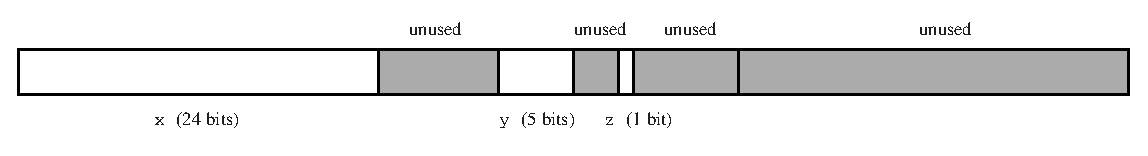
\includegraphics[scale=0.7]{Figures/standardAlignment.eps}\\
% ``Byte'' alignment byte-aligns the object and all fields:
% \hfill\raisebox{-1ex}[0pt][0pt]{\parbox[t]{3in}{
% \begin{samplecode}
% class A \{\\
% \>int x;  /* actual width 24 bits */\\
% \>byte y; /* actual width 5 bits */\\
% \>boolean z; /* actual width 1 bit */\\
% \}\\
% \end{samplecode}
% }}\\
% 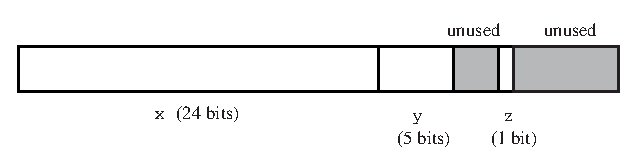
\includegraphics[scale=0.7]{Figures/byteAlignment.eps}\\
% ``Bit'' alignment requires no alignment of objects or fields:\\
% 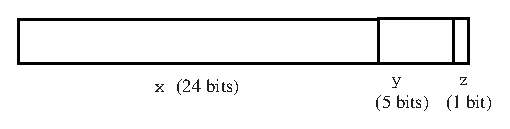
\includegraphics[scale=0.7]{Figures/bitAlignment.eps}\\
% \hline
% \end{tabular}

% Object header omitted.
% \end{slide}

%---------------------------------------------------------------------- SLIDE -
\begin{slide}{Field packing}
% converted with pngtopnm Figures/alignment.png | pnmtops -equalpixels -noturn > Figures/alignment.eps
\begin{center}
\vspace{0.75cm}
%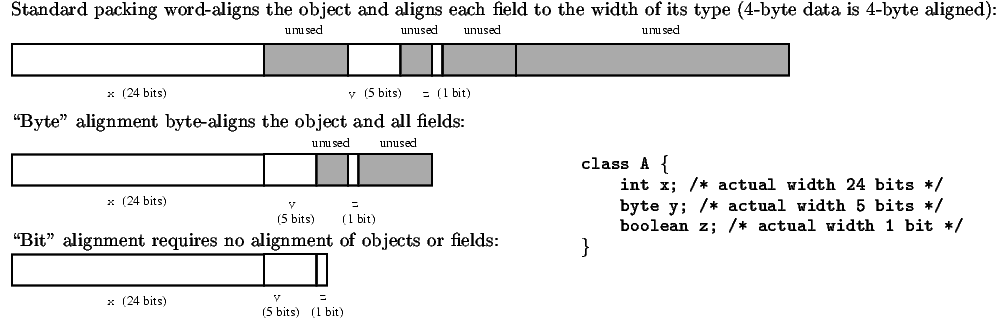
\includegraphics[scale=1.3]{Figures/alignment.eps}
\includegraphics[scale=0.35]{Figures/alignment2.eps}

\small Object header omitted.
\end{center}
\end{slide}

\begin{talknotes}
The actual situtation is a little more complicated.  There is padding
within and at the end of the object, required for various reasons.
The heap allocator may prefer to have the chunks it returns aligned
on certain boundaries, and the machine architecture may prefer to
access, for example, word data aligned at word boundaries.  At
some runtime cost, we can overcome these limitations.  At the top, is
the standard ``Java'' object packing.  All fields are aligned to their
natural size, so that, word-sized fields will always begin at word
boundaries.  In this work we implemented a ``byte'' alignment
strategy, where all fields are placed at the nearest \emph{byte}
boundaries, irrespective of their preferred alignment.  One can also
imagine a ``bit'' alignment strategy where each field uses
\emph{exactly} the number of bits it requires.  At runtime we must
then perform bit-masking and -extraction operations to access the
fields.  We found very little additional space-savings potential from
going to bit alignment, which is why the numbers we will present use
``byte'' alignment.

~%
\end{talknotes}

%---------------------------------------------------------------------- SLIDE -
\begin{slide}{How to compress objects} % just the second one

Three broad techniques:

\parbox[b]{2.5in}{%
\begin{itemize}%
\lightgray\renewcommand{\green}{\lightgray}% new bullet color
\item Field compression
\fieldelim\renewcommand{\green}{\fieldelim}% new bullet color
\item Mostly-constant field elimination
\lightgray\renewcommand{\green}{\lightgray}% new bullet color
\item Header optimizations
\renewcommand{\green}{\yellow} % restore yellow bullet color
\end{itemize}
}%
\parbox[b]{1.75in}{%
\hspace*{0.106in}\includegraphics[scale=0.4]{Figures/Kontour/how-fieldelim-bbox.eps}%
}%
\end{slide}

\begin{talknotes}
Let's return to our outline.  So far we have talked about field
compression; using bitwidth analysis to reduce the static size of
fields allocated in objects, and using field packing to reduce the
amount of object padding.  Now we will talk about ``Mostly-constant
field elimination,'' our second space-reduction technique.
\end{talknotes}

%---------------------------------------------------------------------- SLIDE -
\overlays{6}{
\begin{slide}{Mostly-constant field elimination}
\begin{itemize}
 \item It's easy to remove {\yellow constant} fields.
 \fromSlide{2}{
 \item Key idea: remove \textit{\yellow mostly} constant fields.
 \fromSlide{3}{
 \begin{itemize}
  \item \bp{\yellow Identify} fields which have a certain value ``most of
        the time.''
  \fromSlide{4}{
  \begin{itemize}
   \item \small Static analysis/profiling.
  \end{itemize}
  \fromSlide{5}{
  \item \bp{\yellow Transform} objects to remove fields w/ the common
        value.
  \fromSlide{6}{
  \begin{itemize}
   \item \small Static specialization/externalization.
  \end{itemize}
  }}}
 \end{itemize}
 }}
\end{itemize}
\end{slide}
}

\begin{talknotes}
It's easy to remove constant fields; we just replace the field
reference with the appropriate constant.  @ But our key idea here is
that it is also possible to replace \emph{mostly}-constant fields.
@ We identify fields which have a certain value ``most of the time''
using @ static analysis and profiling.  @ We can then transform the
objects to remove fields with the common value, so that we only
spend space on fields with unusual values.  @ Our techniques for doing
this are called static specialization and externalization.
The types of ``mostly-constant'' fields that can be removed are
slightly different with the two techniques; we will look at static
specialization first.
\end{talknotes}

%---------------------------------------------------------------------- SLIDE -
\overlays{2}{
\begin{slide}{Specialization example:\\\small java.lang.String}
\fontsize{9}{9}%
\newcommand{\myOffset}{\onlySlide*{1}{\makebox[0pt][l]{offset}}\onlySlide{2}{{\yellow getOffset()}}}%
\bfseries\begin{samplecode}%
public final class String \{\\
\>private final char value[];\\
\onlySlide*{2}{\pnode{offl}}%
\>private final int offset;\onlySlide*{2}{\pnode{offr}}\\
\>private final int count;\\
\onlySlide{2}{\>\yellow protected int getOffset() \{ return 0; \}}\\
\>\ldots\\
\>public char charAt(int i) \{\\
\>\>return value[\myOffset{}+1];\\
\>\}\\
\>public String substring(int start) \{\\
\>\>int noff = \myOffset{} + start;\\
\>\>int ncnt = count - start;\\
\>\>return new String(value, noff, ncnt);\\
\>\}\\
\}\\
\end{samplecode}
\onlySlide*{2}{\ncline[linecolor=red,linewidth=2pt]{offl}{offr}}%
\end{slide}
}

\begin{talknotes}
We're going to jump right in with an example.  This is {\tt
  java.lang.String} from the Java standard class library.  It has
three fields: a character array and an integer length and offset.
This representation was chosen to allow you to perform the substring
operation in constant time; you don't have to copy the string, you
just create a new string with a different offset and length and
share the same character array.

The interesting thing about {\tt java.lang.String} is that the {\tt
  offset} field is almost \emph{always} zero.  Only strings created
with the {\tt substring()} method have non-zero offset fields. 
And the offset field is never changed after the object is created.  So
this is a prime opportunity for space reduction.  Here's what we do:
@ we chop out the offset field from the class and replace it with
an accessor method, {\tt getOffset()}, which always returns zero.
All references to the field are made to use the accessor method
instead.
\end{talknotes}

%---------------------------------------------------------------------- SLIDE -
\begin{slide}{Specialization example:\\\small java.lang.String}
\fontsize{9}{9}%
\bfseries\begin{samplecode}%
public final class {\yellow SmallString} \{\\
\>private final char value[];\\
\>\\  
\>private final int count;\\
\>protected int getOffset() \{ return 0; \}\\
\>\ldots\\
\>public char charAt(int i) \{\\
\>\>return value[getOffset()+i];\\
\>\}\\
\>\ldots\\
\}\\
public final class {\yellow BigString extends SmallString} \{\\
\>private final int {\yellow offset};\\
\>protected int {\yellow getOffset()} \{ return offset; \}\\
\}\\
\end{samplecode}
\end{slide}

\begin{talknotes}
Now we're going to call this version of the String class
\emph{SmallString} and we're going to create a subclass
\emph{BigString} which contains the offset field, and where
{\tt getOffset()} works as you'd expect.

Now we have to transform all instantiations of {\tt String} to
refer to the proper version of the class.
\end{talknotes}

%---------------------------------------------------------------------- SLIDE -
\newcommand{\myString}{\onlySlide*{1}{\makebox[0pt][l]{String}}\onlySlide{2}{{\yellow SmallString}}}%
\overlays{2}{
\begin{slide}{Transforming allocation sites}
Case 1: field is constant in constructor.

\fontsize{10}{10}%
\bfseries\begin{samplecode}
\onlySlide*{2}{Small}String s = new \myString(new char[] \{'a', 'b', 'c'\});\\
\\
\myString(char[] val) \{\\
\>this.value = (char[]) val.clone();\\
\onlySlide*{2}{\pnode{offl2}}%
\>this.offset = 0;%
\onlySlide*{2}{\pnode{offr2}}\\
\>this.count = val.length;\\
\}\\
\end{samplecode}
\onlySlide*{2}{\ncline[linecolor=red,linewidth=2pt]{offl2}{offr2}}%
\end{slide}
}

\begin{talknotes}
In some cases, the field is constant in the constructor.  Every
instantiation which uses this constructor will set offset to zero.
(And as we mentioned before, it is never reset after construction.)
So  we juse @ replace the instantiation of {\tt String} with that
of {\tt SmallString}.
\end{talknotes}

%---------------------------------------------------------------------- SLIDE -
\overlays{2}{
\begin{slide}{Transforming allocation sites}
Case 2: field is simple function of constructor parameter.

\fontsize{10}{10}%
\bfseries\begin{samplecode}%
\onlySlide*{1}{%
String s = new String(new char[] \{'a', 'b', 'c'\},\\
~~~~~~~~~~~~~~~~~~~~~~x, 1);\\
\\
String(char[] val, int offset, int length) \{\\
\>this.value = (char[]) val.clone();\\
\>this.offset = offset;\\
\>this.count = length;\\
\}\\
}%
\onlySlide*{2}{%
SmallString s;\\
\\
if (x==0)\\
\>s = new {\yellow SmallString}(new char[] \{'a', 'b', 'c'\}, x, 1);\\
else\\
\>s = new {\yellow BigString}(new char[] \{'a', 'b', 'c'\}, x, 1);\\
}%
\end{samplecode}
\end{slide}
}

\begin{talknotes}
In other cases, the value of the offset field is a simple function of
some parameter given to the constructor.  @ In this case, we will
add a test around the allocation site, so that we can construct
a Small or Big string depending on the value given.  You can imagine a
third case, which doesn't actually show up in {\tt java.lang.String},
where we can obtain \emph{no} usable compile-time information about
the field.  In this case, we always have to create an instance of
{\tt BigString}.
\end{talknotes}

%---------------------------------------------------------------------- SLIDE -
\begin{slide}{Static specialization}
\begin{itemize}
\item Split class implementations into ``field-less'' and
  ``field-ful'' versions.
\item Use virtual accessor functions to hide this split from users of
  the class.
\item Done at compile time, on fields which can be shown to be
  compile-time constants, thus ``static.''
\begin{itemize}
\item Fields can not be mutated after the constructor completes.
\end{itemize}
\item Can be done recursively on multiple fields.
\begin{itemize}
\item Profiling guides splitting order if there are multiple candidates.
\end{itemize}
\end{itemize}
\end{slide}

\begin{talknotes}
This transformation is what we call ``static specialization.''  We
split the class into field-less and field-ful versions, and use
virtual accessor functions to hide the split from users of the class.
This works only on compile-time constant fields which are not mutated
after construction.
We can do this recursively; we use profiling to determine the best
splitting order if we have multiple candidate fields.
\end{talknotes}

%---------------------------------------------------------------------- SLIDE -
\begin{slide}{Creating external fields}
\vspace{1cm}
\begin{itemize}
 \item Sometimes fields are \textit{\yellow run-time} constants (or nearly so)
      but not \textit{\yellow compile-time} constants.
 \begin{itemize}
  \item Examples: sparse matrices, ``two-input nodes'' in Jess expert
        system, the ``next'' field in short linked lists.
 \end{itemize}
 \item \bp{\yellow Exploit field$\rightarrow$map duality} to reduce memory
       overhead in the common case.
\end{itemize}
\end{slide}

\begin{talknotes}
\end{talknotes}

%---------------------------------------------------------------------- SLIDE -
\overlays{3}{
\begin{slide}{Fields and Maps}
\begin{itemstep}
\item Accessing an object field {\tt a.b} (where {\tt a} is the object
  reference and {\tt b} is the field name) is equivalent to evaluating
  a map from \tuple{a, b} to the value type.
\item The mapping we will implement will be \textit{\yellow incomplete}.  We
  define the result of accessing a non-existing mapping to be $\bot$.
\item To achieve our storage savings, we map $\bot$ to the frequent
  ``mostly-constant'' value.
\end{itemstep}
\end{slide}
}

\begin{talknotes}
\end{talknotes}

%---------------------------------------------------------------------- SLIDE -
\overlays{4}{
\begin{slide}{External map implementation}
\centering
\begin{minipage}[c]{0.4\textwidth}
 \centering%
 \vspace{0.5cm}%
 \includegraphics[scale=0.5]{Figures/extmap1.eps}%
 \vspace{0.5cm}%
\end{minipage}%
\begin{minipage}[c]{0.6\textwidth}
 \begin{itemstep}
  \item ``open addressed'' for low overhead.
  \item load-factor of 2/3
  \item two-word key and one-word values means break-even point is 82\%
    \\ \fromSlide{4}{ \tiny (i.e. field may not differ from the
 ``mostly-constant'' value in more than 18\% of objects.)}
 \end{itemstep}
\end{minipage}
\end{slide}
}

\begin{talknotes}
\end{talknotes}

%---------------------------------------------------------------------- SLIDE -
\overlays{4}{
\begin{slide}{We can do better!}
\centering
\begin{minipage}[c]{0.4\textwidth}
 \centering%
 \vspace{0.5cm}%
 \includegraphics[scale=0.5]{Figures/extmap2.eps}%
 \vspace{0.5cm}%
\end{minipage}%
\begin{minipage}[c]{0.6\textwidth}
 \small
 \begin{itemstep}
  \item Use small integers to enumerate fields.
  \item Offset the object pointer by the field index to get a 1-word key.
  \item Limits the number of fields which may be externalized, based
        on the size of the object.
  \item one-word key and one-word value lowers break-even point to 66\%.
 \end{itemstep}
\end{minipage}
\end{slide}
}

\begin{talknotes}
\end{talknotes}

%---------------------------------------------------------------------- SLIDE -
\overlays{3}{
\begin{slide}{Other details}
\begin{itemstep}
\item Use value profiling to identify classes where field
  externalization will be worthwhile.
\item In our experiments, looked for integer ``mostly-constant''
  values in the range $[-5,5]$ for numeric types.  Only looked at {\tt
    null} as a candidate for pointer types.
\item 0 and 1 by far the most common.
\end{itemstep}
\end{slide}
}

\begin{talknotes}
\end{talknotes}

%---------------------------------------------------------------------- SLIDE -
\begin{slide}{How to compress objects} % just the third one

Three broad techniques:

\parbox[b]{2.5in}{%
\begin{itemize}%
\lightgray\renewcommand{\green}{\lightgray}% new bullet color
\item Field compression
\lightgray\renewcommand{\green}{\lightgray}% new bullet color
\item Mostly-constant field elimination
\headeropt\renewcommand{\green}{\headeropt}% new bullet color
\item Header optimizations
\renewcommand{\green}{\yellow} % restore yellow bullet color
\end{itemize}
}%
\parbox[b]{1.75in}{%
\includegraphics[scale=0.4]{Figures/Kontour/how-header-bbox.eps}%
}%
\end{slide}

\begin{talknotes}
\end{talknotes}

%---------------------------------------------------------------------- SLIDE -
\begin{slide}{Header optimizations:\\\small Hashcode/Lock compression}
\begin{center}
\vspace{.5cm}
\includegraphics[scale=0.6]{Figures/Kontour/hashcomp-bbox.eps}
\end{center}
\end{slide}

\begin{talknotes}
\end{talknotes}

%---------------------------------------------------------------------- SLIDE -
\overlays{2}{
\begin{slide}{Header optimizations:\\\small Hashcode/Lock compression}
\begin{itemstep}
\item Implemented as a special case of field externalization.
\item Could also use a static pointer analysis.
\end{itemstep}
\end{slide}
}

\begin{talknotes}
\end{talknotes}

%---------------------------------------------------------------------- SLIDE -
\overlays{3}{
\begin{slide}{Header optimizations:\\\small claz compression}
\begin{itemstep}
\item replace {\tt claz} pointer with a (smaller) table index.
\item With co-operation of GC, works in dynamic environments.
\item Many applications use less than 256 object types.
\end{itemstep}
\end{slide}
}

\begin{talknotes}
\end{talknotes}

%---------------------------------------------------------------------- SLIDE -
\begin{slide}{Header optimizations:\\\small claz compression}
\begin{center}
\includegraphics[scale=0.5]{Figures/Kontour/classcomp-bbox.eps}
\end{center}
\end{slide}

\begin{talknotes}
\end{talknotes}

%---------------------------------------------------------------------- SLIDE -
\begin{slide}{Class statistics}
Class statistics for applications in SPECjvm98 benchmark suite:
\begin{center}
\includegraphics[scale=0.5]{Figures/specclaz.eps}
\end{center}
\end{slide}

\begin{talknotes}
\end{talknotes}

%---------------------------------------------------------------------- SLIDE -
\part{How well does it work?}

\begin{talknotes}
\end{talknotes}

%---------------------------------------------------------------------- SLIDE -
\begin{slide}{Reduction in total live data}
\begin{center}
\includegraphics[scale=0.45]{Figures/oopsla-ttllive-color.eps}
\end{center}
\end{slide}

\begin{talknotes}
\end{talknotes}

%---------------------------------------------------------------------- SLIDE -
\begin{slide}{Reduction in total allocations}
\begin{center}
\includegraphics[scale=0.45]{Figures/oopsla-ttlalloc-color.eps}
\end{center}
\end{slide}

\begin{talknotes}
\end{talknotes}

%---------------------------------------------------------------------- SLIDE -
\begin{slide}{Reduction in object allocations}
\begin{center}
\includegraphics[scale=0.45]{Figures/oopsla-objalloc-color.eps}
\end{center}
\end{slide}

\begin{talknotes}
\end{talknotes}

%---------------------------------------------------------------------- SLIDE -
\begin{slide}{Moderate performance impact}
\begin{center}
\includegraphics[scale=0.45]{Figures/oopsla-speed-color.eps}
\end{center}
\end{slide}

\begin{talknotes}
\end{talknotes}

%---------------------------------------------------------------------- SLIDE -
\overlays{9}{
\begin{slide}{Limitations \\ \small (read, ``future work'')}
\fromSlide{2}{
\begin{itemize}
 \item No array analysis/can't distinguish between different uses of a class.
 \fromSlide{3}{
 \begin{itemize} \yellow\small
  \item Use pointer analysis to discriminate among objects from a
    certain allocation-site; optimize each alloc site.
 \end{itemize}
 \fromSlide{4}{
 \item No pointer compression.
 \fromSlide{5}{
 \begin{itemize} \yellow\small
  \item Investigate region-based/enumerated approaches.
 \end{itemize}
 \fromSlide{6}{
 \item Mostly-constant analysis requires profiling.
 \fromSlide{7}{
 \begin{itemize} \yellow\small
  \item Investigate heuristic methods.
 \end{itemize}
 \fromSlide{8}{
 \item Knows nothing about ``field-like'' maps.
 \fromSlide{9}{
 \begin{itemize} \yellow\small
  \item Enable \emph{internalization}.
 \end{itemize}
 }}}}}}}
\end{itemize}
}
\end{slide}
}

\begin{talknotes}
\end{talknotes}

%---------------------------------------------------------------------- SLIDE -
\begin{slide}{Conclusions}
\begin{itemize}
 \item We achieved substantial space savings on typical
 object-oriented applications.
\end{itemize}
\end{slide}

\begin{talknotes}
\end{talknotes}

%---------------------------------------------------------------------- SLIDE -
\part{The Graveyard Of Unused Slides follows this point.}

\begin{talknotes}
\end{talknotes}

%---------------------------------------------------------------------- SLIDE -
\begin{slide}{Opportunities}
\begin{center}
\includegraphics[scale=0.45]{Figures/spec-space-2.eps}
\end{center}
\end{slide}

\begin{talknotes}
\end{talknotes}

%---------------------------------------------------------------------- SLIDE -
\overlays{3}{
\begin{slide}{Bitwidth analysis}
Motivation:
\begin{itemize}
\item Tedious and error-prone for programmer to manually specify
  widths.
\end{itemize}

\begin{tabular}{lll}%
%\hspace*{0in}&% spacing
\parbox[t]{1.3in}{\begin{mysamplecode}%
\onlySlide*{3}{\pnode{tlx}}%
struct foo \{\\
\>int x:24;\\
\>int y:5;\\
\>int z:1;\\
\};\\
\onlySlide*{3}{\pnode{blx}}~
\end{mysamplecode}
}&%
\parbox[t]{1.3in}{\fromSlide{2}{%
\begin{mysamplecode}%
void foo() \{\\
\>int x:24;\\
\>int y:5;\\
\>int z:1;\\
\>\ldots\\
\}%
\end{mysamplecode}
}}&%
\parbox[t]{1.3in}{\fromSlide{3}{\yellow\begin{mysamplecode}%
\pnode{trx}%
void foo() \{\\
\>int x, y, z;\\
\>\\
\>\ldots\\
\}\\
\pnode{brx}%
~
\end{mysamplecode}
}}\\
\end{tabular}

\fromSlide{3}{
\begin{itemize}
\item The compiler can do it for us!
\end{itemize}
\ncline[linecolor=red,linewidth=3pt]{tlx}{brx}%
\ncline[linecolor=red,linewidth=3pt]{blx}{trx}%
}
\end{slide}
}

\begin{talknotes}
\end{talknotes}

%---------------------------------------------------------------------- SLIDE -
%\begin{slide}{Title here}
%\end{slide}

%\begin{talknotes}
%\end{talknotes}

\end{document}

%%% Local Variables: 
%%% mode: latex
%%% TeX-master: t
%%% End: 
